%Implementierung_dotmul

%\subsubsection{Punktprodukt}

%Im Abb. \ref{Vektor} wird das Implementierungsmethode in CUDA gezeigt. $A$ und $b$ sind Vektoren, die sich miteinander in jeweiligem Thread multipliziert werden müssen. $cs$ sind erzeugte Produktvektoren, die allen zu einem Wert summiert werden. Da eine Beschrankung des CUDA-Blocksizes maximum 512 Threads enthält, muss ein Block iterativ oder mehrere Blocks verwendet werden.

\subsubsection{Skalarprodukt}

Abb. \ref{Vektor} zeigt schematisch eine Skalarprodukt-Implementierung in CUDA:

Der $n$te Thread berechnet das Vektorelement \mbox{ $c_n = a_n \cdot b_n$ }
Die Elemente des Ergebnisvektors $ \bf c $ werden  zu einem Skalar
aufsummiert.
Überschreitet die Vektorgröße die maximale Blockgröße 512 iteriert der Thread
über mehrere Elemente, oder mehrere Blöcke müssen
abgestimmt auf den großen Vektoren arbeiten.


\begin{figure}[htbp]
%\centering
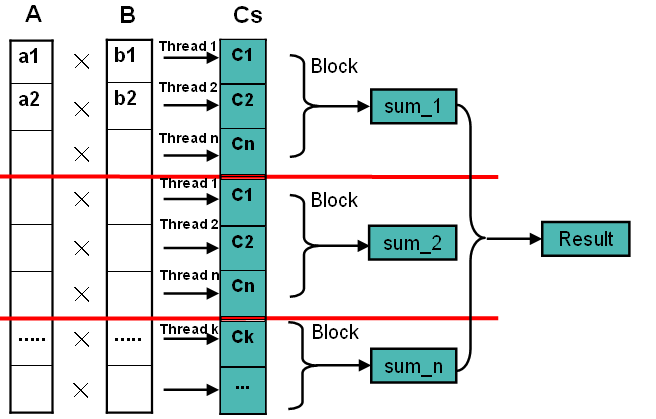
\includegraphics[width=3.5in]{../xby/pic/Vektor}
\caption{ \label{Vektor} Skalaprodukt: Multiplikand $ \bf a$ , Multiplikator $ \bf b$,
\mbox{ (Zwischen-)Ergebnisvektor $\bf c_s$ }}

\end{figure}